\section{Traducci\'on Dirigida por Sintaxis}
\subsection{Atributos}
Para hacer la Traducci\'on Dirigida por Sintaxis, lo primero que hacemos es 
definir los atributos de cada s\'imbolo Terminal y No Terminal.

\begin{center}
  \begin{tabular}{| l | c | r |}
    \hline
    Atributo & Tipo & - \\ \hline
    E.x & int & Heredado \\ \hline
    E.y & int & Heredado \\ \hline
    E.size & int & Heredado \\ \hline
    E.h\_top & int & Sintetizado \\ \hline
    E.h\_buttom & int & Sintetizado \\ \hline
    E.ancho & int & Sintetizado \\ \hline
    
    C.x & int & Heredado \\ \hline
    C.y & int & Heredado \\ \hline
    C.size & int & Heredado \\ \hline
    C.h\_top & int & Sintetizado \\ \hline
    C.h\_buttom & int & Sintetizado \\ \hline
    C.ancho & int & Sintetizado \\ \hline
    
    I.x & int & Heredado \\ \hline
    I.y & int & Heredado \\ \hline
    I.size & int & Heredado \\ \hline
    I.h\_top & int & Sintetizado \\ \hline
    I.h\_buttom & int & Sintetizado \\ \hline
    I.ancho & int & Sintetizado \\ \hline
    
    A.x & int & Heredado \\ \hline
    A.y & int & Heredado \\ \hline
    A.size & int & Heredado \\ \hline
    A.h\_top & int & Sintetizado \\ \hline
    A.h\_buttom & int & Sintetizado \\ \hline
    A.ancho & int & Sintetizado \\ \hline
  \end{tabular}
\end{center}
  

\subsection{Explicaci\'on}
\subsubsection{Atributos}

\begin{itemize}
  \item x e y: Estos atributos contienen la posici\'on del bloque en el eje (x,y).
  \item size: Este atributo representa el tama\~no del bloque.
  \item ancho: En este atributo guardamos el ancho del bloque. Importante para cuando tenemos concatenaci\'on o operaciones con mas de un bloque.
  \item h\_bottom y h\_top: Estos dos atributos son \'utiles cuando aparecen divisiones, h\_bottom es el alto del denominador y h\_top el alto del numerador. En la siguiente imagen se explica mejor.
\end{itemize}

\begin{center}
\includegraphics[width=2.5cm]{bt}
\end{center}
\newpage
\subsubsection{TDS}

Luego la TDS que escribimos es la siguiente:

\begin{center}
\begin{tabular}{ l  l }
  \textbf{S} $\rightarrow$  &\{E.x = 0, E.y = 0, E.size = 1\} \textbf{E}  \\ 
  
  $\textbf{E}_1 \rightarrow $ & $\{E_2.x = E_1.x + (E_1.ancho - E_2.ancho)/2,$ \\
  & $E_2.y = E_1.y - E_1.h\_bottom - (c +0.2)* E_1.Size, E_2.Size = E_1.Size\} \textbf{E}_2 / $\\
  & $\{C.x = E_1.x + (E_1.ancho - C.ancho)/2, C.y = E_1.y + E_1.h\_top, C.Size = E_1.Size\}\textbf{C}$  \\
  & $\{E_1.h\_top = E_2.h\_top +  E_2.h\_bottom, E_1.h\_bottom = C.h\_bottom + C.h\_top, $ \\
  & $E_1.ancho = max(c.ancho, E_2.ancho)\}$ \\ \\
  
  $\textbf{E} \rightarrow$  &  $\{C_1.x = C_0.x,C_1.y = C_0.y,C_1.Size = C_0.Size\} \textbf{C} $ \\
  & $\{E.ancho = C_1.ancho, E.h\_top = C_1.h\_top, E.h\_bottom = C_1.h\_bottom\}$\\ 
  
  $\textbf{C}_0 \rightarrow$  &  $\{C_1.x = C_0.x,C_1.y = C_0.y,C_1.Size = C_0.Size\}\textbf{C}_1 $ \\
  & $\{I.x = C_0.x + C_1.width, I.y = C_0.y , I.Size = C_0.size\}\textbf{I}$ \\
  & $\{C_0.h\_top = max(C_1.h\_top, C_1.h\_bottom), C_0.h\_bottom = max(C_1.h\_top, C_1.h\_bottom),$ \\
  & $C_0.ancho = C_1.ancho + I.ancho \}$ \\ 
  
  \textbf{C} $\rightarrow$  & $\{I.x = C.x,I.y = C.y,I.Size = C.Size\} \textbf{I} $ \\
  & $\{C.ancho = I.ancho, C.h\_top = I.h\_top, C.h\_bottom = I.h\_bottom\}$\\ 

  
  $\textbf{I} \rightarrow$  &  $\{A_1.x = I.x, A_1.y = I.y , A_1.Size = I.Size\} \textbf{A}_1 $ \\
  &  \textbf{\^{}} $ \{ A_2.x = I.x + A_1.width,  A_2.y = I.y + 0.5*A_2.h\_top ,$\\
  & $A_2.Size = A_1.Size * 0.7\} \textbf{A}_2$ \\
  & $\{I.h\_top = A_1.h\_top, I.h\_bottom = A_1.h\_bottom +A_2.h\_bottom + A_2.h\_top * 0.5, $ \\
  & $I.ancho = A_1.ancho + A_2.ancho \}$\\ \\
  

  
  $\textbf{I} \rightarrow$  &  $\{A_1.x = I.x, A_1.y = I.y , A_1.Size = I.Size\}\textbf{A}_1$ \\
  & $\textbf{\_}  \{ A_2.x = A_1.ancho + I.x,  A_2.y = I.y + 0.5 * A_2.h\_top, A_2.Size = A_1.Size * 0.7\} \textbf{A}_2$ \\
  & $\{I.h\_top = A_1.h\_top, I.h\_bottom = A_1.h\_bottom + A_2.h\_bottom + A_2.h\_top * 0.5, $ \\
  & $ width = A_1.width + A_2.width \}$ \\ 
  

        
        
        
  \textbf{I} $\rightarrow$  &  $\{A_1.size =  I.size, A_1.x = I.x, A_1.y = I.y \}$ \textbf{$A_1$}\^{} \\
  & $ \{  A_2.size = I.size*0.7, A_2.x = I.x + A_1.width, $ \\
  & $ A_2.y = I.y - A_1.h\_top - 0.5 * A_2.h\_bottom + 0.5 * A_2.size \}$ \textbf{$A_2$} \_ \\ 
  & $ \{ A_3.size =  I.size*0.7, A_3.x = I.x + A_1.width, A_3.y = I.y + 0.5*A_3.h\_top \}$ \textbf{$A_3$}  \\
  & $ \{I.h\_top = A_1.h\_top + A_2.h\_top + 0.5 * A_2.h\_bottom - A_2.size * 0.5, $ \\
  & $ I.h\_bottom = A_1.h\_bottom + A_3.h\_bottom + A_3.h\_top * 0.5, $ \\
  & $ I.width =   A_1.width + max(A_2.width, A_3.width)  \}$\\ \\

  
 \textbf{I} $\rightarrow$  & $\{A_1.size = I.size, A_1.x = I.x, A_1.y = I.y\} \textbf{$A_1$}$\_ \\
 & $\{A_2.size = I.size*0.7, A_2.x = I.x + A_1.width, A_2.y= I.y + 0.5 * A_2.h\_top\}\textbf{$A_2$}$ \^{} \\
 &$\{A_3.size =  I.size*0.7, A_3.x = I.x + A_1.width, $ \\
 & $A_3.y = I.y - A_1.h\_top - 0.5 * A_3.h\_bottom + 0.5 * A_3.size\}$$\textbf{$A_3$}$ \\
 & $\{I.h\_top = A_1.h\_top + A_2.h\_top + 0.5 * A_3.h\_bottom - A_3.size * 0.5,  $ \\
 & $I.h\_bottom = A_1-h\_bottom + A_2.h\_bottom + A_2.h\_top * 0.5, $ \\
 & $ I.width = A_1.width + max(A_2.width, A_3.width)\}$ \\ \\
  
  
  \textbf{I} $\rightarrow$  &  \{A.x = I.x, A.y = I.y, A.Size = I.Size\}\textbf{A} \\
  & \{I.h\_top = A.h\_top, I.h\_bottom = A.h\_bottom, I.ancho = A.ancho\} \\ \\ 
  
  \textbf{A} $\rightarrow$ &  \textbf{\{} \{E.x = A.x, E.y = A.y, E.Size = A.Size\}\textbf{E} \\
  & \{A.h\_top = E.h\_top, A.h\_bottom = E.h\_bottom, A.ancho = E.ancho\} \textbf{\}} \\ 
  

        
  \textbf{A} $\rightarrow$ &   \textbf{(}\{E.x = A.x + 0.6*A.size, E.y = A.y, E.Size = A.Size\}\textbf{E} \\
  & \{A.h\_top = E.h\_top, A.h\_bottom = E.h\_bottom, A.ancho = E.ancho + 2*A.size*0.6\}\textbf{)}  \\ 
  
  \textbf{A} $\rightarrow$ &  $\textbf{L} \{A.h\_top = A.size, A.h\_bottom = 0, A.ancho = 0.6 * A.size.\}$\\
  

\end{tabular}
\end{center}

\subsection{Implementaci\'on TDS}
\subsubsection{Reglas Sint\'acticas}
Para implementar las Reglas Sint\'acticas \textbf{ply} nos pide que las definamos de una forma especial, como por ejemplo:

\begin{algorithm}[H]
 def $p\_expression\_divide(p)$: \\
    'expression : expression DIVIDE concatenation' \\
    p[0] = DivisionNode(p[1], p[3])
    \caption{Ejemplo de Regla Sint\'actica}
\end{algorithm}

En el ejemplo se puede ver la regla sint\'actica para la division. Entre ' ' definimos la producci\'on para la queremos esta regla y luego con el par\'ametro P hacemos referencia a cada Terminal/No Terminal de la producci\'on. 
Utilizamos DivisionNode que es una clase de nuestro Arbol Sint\'actico
\subsubsection{\'Arbol Sint\'actico}
Para poder implementar la TDS generamos el una estructura de \textbf{Arbol Sint\'actico}, en la cual tenemos la clase nodo y cada nodo hace referencia a sus hijos y a su padre. Definimos nodos unarios, binarios y ternarios para utilizar dependiendo la cantidad de hijos que necesit\'abamos.
Con esto logramos generar un \textbf{Arbol Sint\'actico} como por ejemplo para la cadena A\_B/C\^{}D, el \'arbol quedar\'ia:
\begin{center}
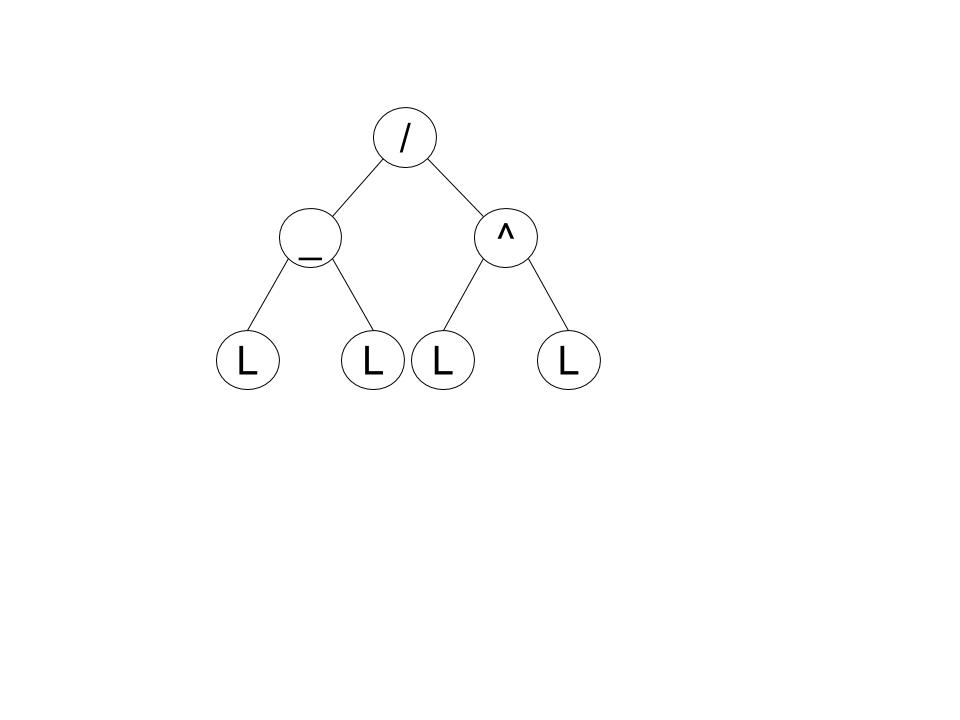
\includegraphics[width=10.5cm]{arbols}
\end{center}

\newpage

\subsection{Recorrido del \'Arbol Sint\'actico}
Para recorrer el \'Arbol Sint\'actico lo que hacemos es separar en tres etapas:

\begin{itemize}
  \item first\_top\_down\_action: En esta funci\'on lo que tenemos que hacer es heredar Size hasta las hojas entonces desde el nodo ra\'iz vamos pasando el atributo \textbf{size} hasta llegar a una hoja
  \item bottom\_up\_action: Una vez con Size en las hojas, sintetizamos \textbf{width}, \textbf{heightTop}, \textbf{heighBot}, hasta la ra\'iz del \'arbol.
  \item second\_top\_down\_action: Por \'ultimo, nos queda heredar \textbf{x} e \textbf{y} entonces, los bajamos hasta las hojas.
\end{itemize}

Una vez terminado estos tres pasados tenemos los atributos acomodados correctamente en el \'arbol sint\'actico.
